\documentclass{beamer}

% Required packages
\usepackage{xcolor}
\usepackage{tikz}
\usepackage{amsmath}
\usepackage{listings}
\usepackage{graphicx}

% Set image search paths
\graphicspath{{../images/}{../../shared/images/}}

% Define custom colors
\definecolor{ds9blue}{RGB}{25,25,112}
\definecolor{ds9gold}{RGB}{218,165,32}
\definecolor{ds9grey}{RGB}{105,105,105}
\definecolor{ds9red}{RGB}{178,34,34}

% Theme configuration
\usetheme{Madrid}
\usecolortheme{whale}
\setbeamercolor{structure}{fg=ds9blue}
\setbeamercolor{alerted text}{fg=ds9red}
\setbeamercolor{example text}{fg=ds9gold}

% Title page configuration
\title[Prompt Engineering]{Computer Science 12: Prompt Engineering Guide}
\subtitle{Effective AI Communication for CS Students}
\author[Mr. Gullo]{Mr. Gullo}
\date[Feb 2025]{February, 2025}
\institute[CS Dept.]{Department of Computer Science}

\begin{document}

% Title page
\frame{\titlepage}

% Table of contents
\begin{frame}
\frametitle{Overview}
\tableofcontents
\end{frame}

% Core Principles
\section{Core Principles}
\frame{\sectionpage}
\begin{frame}
\frametitle{Core Principles}
This guide combines principles from Google's 10 Hour Prompting Essentials and Anthropic's prompting framework:

\begin{block}{Five-Step Framework}
\begin{enumerate}
\item \textbf{Task:} Clearly define what you want the AI to do
\item \textbf{Context:} Provide relevant background information
\item \textbf{References:} Incorporate examples to clarify your needs
\item \textbf{Evaluate:} Assess the AI's output
\item \textbf{Iterate:} Refine your prompt based on evaluation
\end{enumerate}
\end{block}
\end{frame}

\begin{frame}
\frametitle{Prompting Techniques}
\begin{block}{Key Techniques from Emergent Capabilities}
\begin{itemize}
\item \textbf{Role Setting:} Encourage the AI to take on the characteristics of an expert in the chosen task
\item \textbf{Chain of Thought Reasoning:} Prompt the LLM to explicitly state its reasoning process step by step before answering to allow for more thorough and well-reasoned responses to complex queries
\end{itemize}
\end{block}
\end{frame}

\section{CS-Specific Examples}
\frame{\sectionpage}

\begin{frame}
\frametitle{Using References in Your Prompts: Part 1}
\begin{block}{Example: Floating Point Precision}
\textbf{Prompt with Reference:}
\begin{itemize}
\item "You are a CS tutor helping me understand floating point precision issues. Here's my code that's giving wrong results:

\texttt{float result = 0.1 + 0.2;}\\
\texttt{if (result == 0.3)}\\
\texttt{\quad cout << "Equal";}\\
\texttt{else}\\
\texttt{\quad cout << "Not equal";}

Please explain why it prints 'Not equal' and how I should fix it."
\end{itemize}
\end{block}

\begin{alertblock}{Why This Works Better}
\begin{itemize}
\item Provides concrete code example showing the problem
\item Demonstrates specific behavior that needs explanation
\item Gives the AI context about your current understanding
\end{itemize}
\end{alertblock}
\end{frame}

\begin{frame}
\frametitle{Using References in Your Prompts: Part 2}
\begin{block}{Example: Number System Conversion}
\textbf{Prompt with Reference:}
\begin{itemize}
\item "You are a CS tutor helping with number systems. I'm trying to convert between number systems but getting confused. Here are my attempts:

\texttt{Decimal 42 to binary: 00110010}\\
\texttt{Hexadecimal 0x2A to decimal: 52}

Please explain where I went wrong and show the correct conversions with the steps clearly laid out."
\end{itemize}
\end{block}

\begin{alertblock}{Why This Works Better}
\begin{itemize}
\item Shows specific examples of your work
\item Highlights misconceptions that need correction
\item Asks for step-by-step explanation alongside the answer
\item Focuses the AI on educational value, not just giving answers
\end{itemize}
\end{alertblock}
\end{frame}
\begin{frame}
\frametitle{Floating Point Example}
\begin{block}{Weak vs. Optimized Prompts}
\textbf{Weak Prompt:} 
\begin{itemize}
\item "Explain floating point numbers."
\end{itemize}

\textbf{Optimized Prompt:}
\begin{itemize}
\item "You are an expert in teaching computer number systems. Explain the IEEE 754 floating point standard, including the differences between single and double precision. Show the bit layout for each format and walk through an example of how a decimal number is converted to its floating point representation. Include common precision issues that arise in calculations. Act as a CS professor."
\end{itemize}
\end{block}

\begin{alertblock}{Breakdown}
\begin{itemize}
\item Task: Explain floating point representation
\item Context: IEEE 754 standard with examples
\item Role Setting: Act as a CS professor
\end{itemize}
\end{alertblock}
\end{frame}

\begin{frame}
\frametitle{Memory Usage Example}
\begin{block}{Weak vs. Optimized Prompts}
\textbf{Weak Prompt:}
\begin{itemize}
\item "How does computer memory work?"
\end{itemize}

\textbf{Optimized Prompt:}
\begin{itemize}
\item "You are an expert in teaching computer architecture. Explain memory usage in C++ programs, including the stack vs. heap allocation, memory leaks, and efficient memory management techniques. Include code examples that demonstrate proper and improper memory usage. Discuss how different data structures impact memory efficiency. Think step-by-step."
\end{itemize}
\end{block}

\begin{alertblock}{Breakdown}
\begin{itemize}
\item Task: Explain memory usage with practical focus
\item Context: C++ programming environment
\item Role Setting: Expert in teaching computer architecture
\end{itemize}
\end{alertblock}
\end{frame}

\begin{frame}
\frametitle{Number Systems Example}
\begin{block}{Weak vs. Optimized Prompts}
\textbf{Weak Prompt:}
\begin{itemize}
\item "Explain binary numbers."
\end{itemize}

\textbf{Optimized Prompt:}
\begin{itemize}
\item "You are an expert in teaching number systems. Explain binary, octal, and hexadecimal number systems, and show the conversion process between them. Include bitwise operations (AND, OR, XOR, shifts) with examples of when they're useful in programming. Demonstrate how these concepts are applied in C++ code examples. Think step-by-step."
\end{itemize}
\end{block}
\end{frame}

\section{Use Cases for CS Students}
\frame{\sectionpage}
\begin{frame}
\frametitle{Math Libraries Implementation}
\begin{exampleblock}{Example Prompt}
"You are an expert in C++ programming. Explain how to use the C++ math library for solving complex calculations. Show how to implement common mathematical functions like logarithms, trigonometric functions, and exponents. Provide code examples that demonstrate error handling and precision considerations. Think step-by-step about the potential pitfalls students might encounter."
\end{exampleblock}
\end{frame}

\begin{frame}
\frametitle{Input Validation with cin}
\begin{exampleblock}{Example Prompt}
"You are an expert in C++ input/output operations. Demonstrate robust input validation techniques using cin for user input. Show how to handle different types of input (integers, floating-point, strings), deal with buffer issues, and recover from input errors. Include examples of common pitfalls and their solutions. Write code that handles edge cases gracefully. Think step-by-step."
\end{exampleblock}
\end{frame}

\begin{frame}
\frametitle{If/Else and Truth Tables}
\begin{exampleblock}{Example Prompt}
"You are an expert in teaching boolean logic and control flow. Explain the relationship between truth tables and if/else statements in programming. Demonstrate how to implement complex logical conditions using AND, OR, and NOT operators. Show how to simplify boolean expressions and convert them to efficient code. Include examples of common logical errors and debugging techniques. Think step-by-step."
\end{exampleblock}
\end{frame}

\section{Safety and Ethics}
\frame{\sectionpage}
\begin{frame}
\frametitle{Academic Integrity and Safety Guidelines}
\begin{block}{Academic Integrity}
\begin{itemize}
\item Do not use AI to complete assignments or exams without understanding the underlying concepts
\item Use it as a tool to deepen understanding and check work
\end{itemize}
\end{block}

\begin{alertblock}{Common Pitfalls}
\begin{itemize}
\item Avoid oversimplification: AI can provide oversimplified answers that lack nuance
\item Always critically evaluate the AI's output
\item Consult multiple sources to ensure accuracy
\end{itemize}
\end{alertblock}
\end{frame}

\section{LLM Selection for Computer Science}
\frame{\sectionpage}

\begin{frame}
\frametitle{Choosing the Right LLM for CS Tasks}

\begin{block}{Best Practices}
\begin{itemize}
\item Match LLM strengths to specific tasks
\item Consider using multiple models for different use cases
\item Verify outputs against known CS principles
\item Use benchmarks as guidelines, not absolute measures
\end{itemize}
\end{block}
\begin{figure}
    \centering
    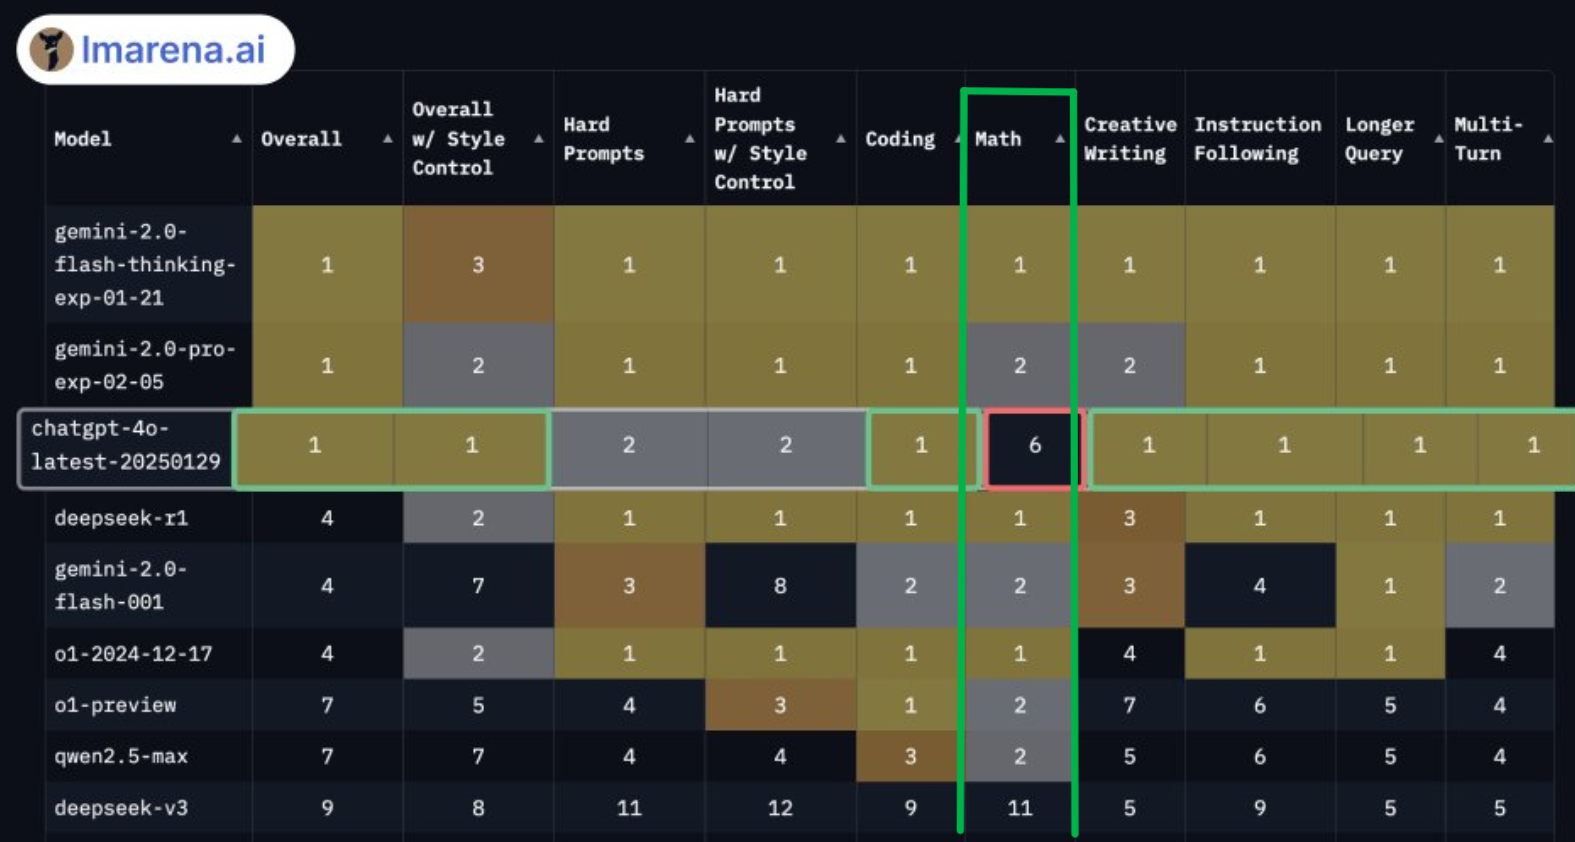
\includegraphics[width=1\linewidth]{cs12-ai-model-benchmarks-lmarena.png}
\end{figure}
\end{frame}

\section{OpenStax-Gemini Partnership (Deprecated?)}
\frame{\sectionpage}

\begin{frame}
\frametitle{OpenStax Integration with Google Gemini}

\begin{block}{Accessing Trustworthy Educational Content}
\begin{itemize}
\item OpenStax has partnered with Google to integrate their library with Gemini (August 2024)
\item 70+ openly licensed, peer-reviewed textbooks now accessible via Gemini
\item Available to Gemini users 18+ in the United States
\end{itemize}
\end{block}

\begin{exampleblock}{How to Access}
\begin{center}
\texttt{@OpenStax explain the concept of object-oriented programming?}
\end{center}
\end{exampleblock}

\begin{alertblock}{Benefits for CS Students}
\begin{itemize}
\item Accurate, attribution-based responses for CS concepts
\item Integration with other Gemini AI capabilities
\item Ensures academic integrity while using AI tools
\end{itemize}
\end{alertblock}
\end{frame}

\begin{frame}
\frametitle{OpenStax and AI in Education}

\begin{columns}
\column{0.5\textwidth}
\begin{block}{Core Principles}
\begin{itemize}
\item Accuracy in educational content
\item Proper attribution to sources
\item Accessibility for all learners
\item Preservation of academic integrity
\end{itemize}
\end{block}

\column{0.5\textwidth}
\begin{alertblock}{Quote}
\small ``OpenStax and Google share a unified, responsible vision for the use of AI in education. We believe content provided through AI learning tools should be accurate and inclusive.''
\begin{flushright}
\scriptsize — Professor Richard G. Baraniuk,\\founder and director of OpenStax
\end{flushright}
\end{alertblock}
\end{columns}

\vspace{0.5cm}
\begin{block}{Impact for CS Education}
\begin{itemize}
\item Access to high-quality CS textbooks through a conversational AI
\item Support for challenging programming concepts with trusted content
\item Democratizing access to educational resources
\end{itemize}
\end{block}
\end{frame}

\section{Using Anthropic's Console}
\frame{\sectionpage}

\begin{frame}
\frametitle{Using Anthropic's Console}
\begin{figure}
    \centering
    \includegraphics[width=1\linewidth]{cs12-prompt-anthropic_console.png}
\end{figure}
\end{frame}

\begin{frame}
\frametitle{Available Advanced Tools}
\begin{enumerate}
\item \textbf{Prompt Optimizer}
\begin{itemize}
\item Utilize the prompt optimizer to refine prompts
\item Improve performance through suggested modifications
\end{itemize}

\item \textbf{Prompt Generator}
\begin{itemize}
\item Create production-ready prompt templates
\item Describe desired task and output format
\end{itemize}

\item \textbf{Test Cases}
\begin{itemize}
\item Generate automatic test cases
\item Compare outputs side by side
\item Facilitate rapid iteration and refinement
\end{itemize}
\end{enumerate}
\end{frame}
\section{XML Tags in Prompting}
\frame{\sectionpage}

\begin{frame}
\frametitle{Using XML Tags in Prompts (!Advanced!)}

\begin{block}{Purpose of XML Tags}
\begin{itemize}
\item Structure content in a clear, machine-readable format
\item Separate different types of information
\item Make prompts more organized and specific
\end{itemize}
\end{block}

\begin{exampleblock}{Common XML Tag Examples}
\begin{itemize}
\item \texttt{<task>}Define specific instructions\texttt{</task>}
\item \texttt{<context>}Provide background information\texttt{</context>}
\item \texttt{<example>}Show sample content\texttt{</example>}
\item \texttt{<output>}Specify desired format\texttt{</output>}
\end{itemize}
\end{exampleblock}

\end{frame}

\section{Additional LLM Tools}
\frame{\sectionpage}

\begin{frame}
\frametitle{Exploring Other LLM Research Tools}

\begin{block}{Alternative AI Research Assistants}
\begin{description}
\item[Perplexity] \hfill \\
   \begin{itemize}
   \item Real-time search integration
   \item Academic paper analysis
   \item Direct citation capabilities 
   \item Built-in fact-checking
   \end{itemize}
   
\item[Google or OpenAI: Deep Research] \hfill \\
   \begin{itemize}
   \item Specialized for academic research
   \item Literature review assistance
   \item Paper summarization
   \item Research methodology guidance
   \end{itemize}
\end{description}
\end{block}


\end{frame}

\begin{frame}
\frametitle{Popular AI-Powered IDEs in 2025}

\begin{block}{AI-Enhanced Development Environments}
\begin{enumerate}
\item \textbf{Windsurf}: Known for its deep integration with project management tools and CI/CD pipelines, offering features like agent mode for hands-free coding sessions and seamless API integration.

\item \textbf{Cursor}: Offers advanced AI assistance for coding, providing real-time suggestions and code completion.

\item \textbf{GitHub Copilot}: A widely used AI-powered tool that assists developers by suggesting code and completing tasks based on context.

\item \textbf{Trae AI}: An IDE that utilizes automated assistance and code generation to enhance software development.

\item \textbf{Replit}: Evolved into a comprehensive AI-powered development environment with features like real-time collaboration and built-in hosting.
\end{enumerate}
\end{block}
\end{frame}


\begin{frame}
\frametitle{Summary}
\begin{itemize}
\item Apply the five-step framework for effective prompts
\item Use role setting and chain of thought reasoning
\item Create detailed, context-rich prompts for CS problems
\item Maintain academic integrity while using AI tools
\item Leverage Anthropic's Console for prompt optimization
\item Always verify and cross-reference AI-generated content
\end{itemize}
\end{frame}

\section{Sources}
\frame{\sectionpage}

\begin{frame}[allowframebreaks]
\frametitle{Sources \& References}

\begin{block}{Core Resources}
\begin{itemize}
\item Google's 10 Hour Prompting Essentials Course\\
    \texttt{https://grow.google/prompting-essentials/}
\item OpenStax and Google Gemini Partnership\\
    \texttt{https://openstax.org/blog/press-release-openstax-partners-googles-gemini-apps}
\item LM Arena Chatbot Leaderboard\\
    \texttt{https://lmarena.ai/?leaderboard}
\end{itemize}
\end{block}

\begin{block}{Additional Tools \& Guides}
\begin{itemize}
\item Google Gemini for Education\\
    \texttt{https://gemini.google.com/education}
\item OpenStax Free Textbooks\\
    \texttt{https://openstax.org}
\item MIT Sloan Effective Prompts Guide\\
    \texttt{https://mitsloanedtech.mit.edu/ai/basics/effective-prompts/}
\end{itemize}
\end{block}
\end{frame}

\begin{frame}
\begin{figure}
    \centering
    \includegraphics[width=1\linewidth]{../images/cs12-prompt-anthropic_console.png}
\end{figure}
\end{frame}
\end{document}